\documentclass[aspectratio=169]{beamer}

\usepackage[utf8]{inputenx} % For æ, ø, å
\usepackage{csquotes}       % Quotation marks
\usepackage{microtype}      % Improved typography
\usepackage{amssymb}        % Mathematical symbols
\usepackage{mathtools}      % Mathematical symbols
\usepackage[absolute, overlay]{textpos} % Arbitrary placement
\setlength{\TPHorizModule}{\paperwidth} % Textpos units
\setlength{\TPVertModule}{\paperheight} % Textpos units
\usepackage{tikz}
\usetikzlibrary{overlay-beamer-styles}  % Overlay effects for TikZ

\AtBeginSection{\frame{\sectionpage}}
\AtBeginSubsection{\frame{\subsectionpage}}

\usepackage{hyperref}
\usepackage{svg}
%\usefonttheme{serif}

\usepackage{xfrac}
\usepackage{color, soul, xcolor} % Colored text and highlighting, respectively
\makeatletter
\let\HL\hl
\renewcommand\hl{%
  \let\set@color\beamerorig@set@color
  \let\reset@color\beamerorig@reset@color
  \HL}
\makeatother
\usepackage{tikz-cd} % For commutative diagrams
\usepackage{tikz-3dplot}
\usetikzlibrary{angles}
\RequirePackage{pgfplots}
\usepackage{mathtools}
\usepackage{answers}
\usepackage{setspace}
\usepackage{graphicx}
\usepackage{enumerate}
\usepackage{multicol}
\usepackage{mathrsfs}
\usepackage{amsmath,amsthm,amssymb}
\usepackage{marvosym,wasysym} %fucking smileys
\usepackage{float}
\usepackage{morefloats}
\usepackage{pgf,tikz}
\pgfplotsset{compat=1.15}
\usepackage{mathrsfs}
\usetikzlibrary{arrows}
\usepackage{subcaption}
\usepackage[most]{tcolorbox}
\tcbuselibrary{theorems}
\usepackage{fancyvrb}
\usepackage{longtable,booktabs}
\usepackage{stackrel}
\usepackage{animate}
\usepackage[percent]{overpic}
\definecolor{lighter_csu_green}{RGB}{60,133,77}
\newcommand\boldgreen[1]{\textcolor{lighter_csu_green}{\emph{\textbf{#1}}}}
\usepackage{MnSymbol}
%border matrix
\makeatletter
\newif\if@borderstar
\def\bordermatrix{\@ifnextchar*{%
\@borderstartrue\@bordermatrix@i}{\@borderstarfalse\@bordermatrix@i*}%
}
\def\@bordermatrix@i*{\@ifnextchar[{\@bordermatrix@ii}{\@bordermatrix@ii[()]}}
\def\@bordermatrix@ii[#1]#2{%
\begingroup
\m@th\@tempdima8.75\p@\setbox\z@\vbox{%
\def\cr{\crcr\noalign{\kern 2\p@\global\let\cr\endline }}%
\ialign {$##$\hfil\kern 2\p@\kern\@tempdima & \thinspace %
\hfil $##$\hfil && \quad\hfil $##$\hfil\crcr\omit\strut %
\hfil\crcr\noalign{\kern -\baselineskip}#2\crcr\omit %
\strut\cr}}%
\setbox\tw@\vbox{\unvcopy\z@\global\setbox\@ne\lastbox}%
\setbox\tw@\hbox{\unhbox\@ne\unskip\global\setbox\@ne\lastbox}%
\setbox\tw@\hbox{%
$\kern\wd\@ne\kern -\@tempdima\left\@firstoftwo#1%
\if@borderstar\kern2pt\else\kern -\wd\@ne\fi%
\global\setbox\@ne\vbox{\box\@ne\if@borderstar\else\kern 2\p@\fi}%
\vcenter{\if@borderstar\else\kern -\ht\@ne\fi%
\unvbox\z@\kern-\if@borderstar2\fi\baselineskip}%
\if@borderstar\kern-2\@tempdima\kern2\p@\else\,\fi\right\@secondoftwo#1 $%
}\null \;\vbox{\kern\ht\@ne\box\tw@}%
\endgroup
}
\makeatother

\usetheme{UiB}

%For easier reading
\setbeamersize{text margin left=40pt,text margin right=40pt}
\renewcommand{\baselinestretch}{1.3}


%% FONT STUFF
\usepackage{amsmath}
\usepackage{amsfonts}
\usefonttheme[onlymath]{serif}

%Commands
\newcommand{\R}{\mathbb{R}}
\newcommand{\C}{\mathbb{C}}
\newcommand{\opens}{\mathcal{O}}
\newcommand{\hilbert}{\mathcal{H}}
\newcommand{\algebra}{\mathcal{A}}
\newcommand{\ideals}{\mathcal{I}}
\newcommand{\functionals}{\mathcal{M}}
\newcommand{\spec}{\mathrm{spec}}
\newcommand{\clifford}{\mathrm{C}\ell}
    \newcommand\quotient[2]{
        \mathchoice
            {% \displaystyle
                \text{\raise1ex\hbox{$#1$}\Big/\lower1ex\hbox{$#2$}}%
            }
            {% \textstyle
                #1\,/\,#2
            }
            {% \scriptstyle
                #1\,/\,#2
            }
            {% \scriptscriptstyle  
                #1\,/\,#2
            }
    }


\author{Colin Roberts}
\setbeamercolor{title}{fg=white} 
\title{The Calder\'on Problem}
\setbeamercolor{subtitle}{fg=white} 
\subtitle{on Riemannian Manifolds}



\begin{document}


\begin{frame}{}
\vfill
In 1980, Alberto Calder\'on proposed a problem in his paper \emph{On an inverse boundary value problem}. 
\pause
    \begin{itemize}
        \item He wanted to know if one can determine the conductivity of a domain by making voltage and current measurements along the boundary.
        
        \pause
        \item This is the Electrical Impedence Tomography problem.
        
        \pause
        \item Originally his motivation was for oil prospecting. 
        
        \pause
        \item This problem sparked interest due to its usefulness in geophysical and medical imaging.
    \end{itemize}
\vfill
\end{frame}

\begin{frame}{}
\vfill
\begin{figure}[H]
    \centering
    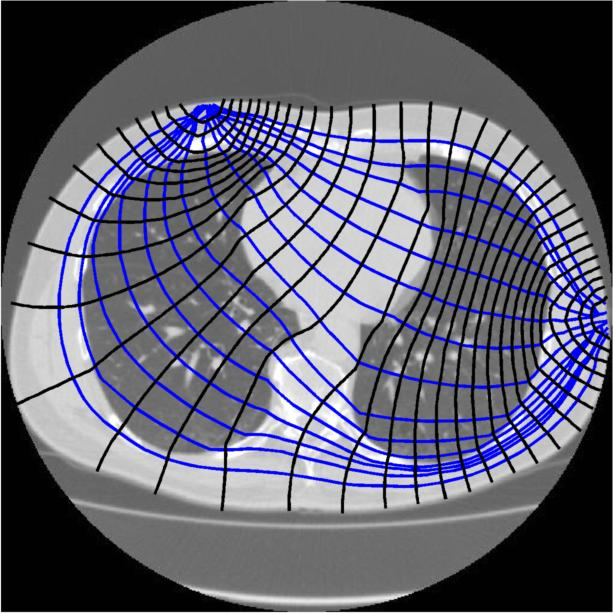
\includegraphics[width=.5\textwidth]{eit.jpg}
\end{figure}
\vfill
\end{frame}

\begin{frame}{}
\vfill
The two main groups working on this problem now are... 
\pause
    \begin{itemize}
        \item Practitioners: Work with incomplete and noisy data to recover information in the real world.
        
        \pause
        \item Theorists: Work in ideal scenarios with a chosen amount of information to see the scope of possibilities.
    \end{itemize}
\vfill    
\end{frame}

\begin{frame}{}
\vfill
The two main groups working on this problem now are... 
    \begin{itemize}
        \item Practitioners: Work with incomplete and noisy data to recover information in the real world.
        
        \item \hl{Theorists: Work in ideal scenarios with a chosen amount of information to see the scope of possibilities.}
    \end{itemize}
\vfill
\end{frame}

\begin{frame}{Problem Statement}
\vfill
    \textbf{\underline{Idea:}} Given a domain $\Omega$ with interior $\Omega^+$ that we cannot probe, can we determine the conductivity $\gamma$ matrix by studying the boundary $\partial \Omega$? 
    \pause
    \begin{itemize}
        \item $\Omega^+$ is free of charges, hence $\nabla \cdot (\gamma \nabla u) = 0$ in $\Omega^+$ where $u$ is the electrostatic potential.
        
        \pause
        \item Apply a known voltage $f$ at the boundary $\partial \Omega$. Hence $f = u \vert_{\partial \Omega}$.
        
        \pause
        \item Measure the current flux $h$ through the boundary $\partial \Omega$. Hence, $h = \frac{\partial u}{\partial \nu}$.
        
        \pause
        \item This defines the voltage-to-current map $\Lambda$ so that $\Lambda(f) = h$.
        
        \pause
        \item Can we determine the conductivity matrix $\gamma$ from $\Lambda$?
    \end{itemize}
\vfill
\end{frame}


\begin{frame}{On Manifolds}
\vfill 
    \begin{itemize}
        \pause
        \item Let (unknown) connected $\Omega$ be a smooth compact Riemannian manifold with boundary $\partial \Omega$.
        
        \pause
        \item Replace conductivity be represented by (unknown) $g$ since $\gamma^{jk}=\sqrt{|g|}g^{jk}$.
        
        \pause
        \item Let $\Delta u = 0$ in $\Omega^+$ and $u=f$ on $\partial \Omega$, with $\Delta$ the Hodge-Laplacian $d\delta+\delta d$.
        
        \pause
        \item \boldgreen{Dirichlet-to-Neumann operator} $\Lambda$ maps Dirichlet data $f=u|_{\partial \Omega}$ to $g = \frac{\partial u}{\partial \nu}=\iota^*(\star d u)$.
        
        \pause
        \item Recover $g$ from knowing $\Lambda$.
        
        \pause
        \item The EIT problem and the Calder\'on problem on manifolds are equivalent in dimensions $n\neq 2$.
    
    \end{itemize}
\vfill
\end{frame}



\end{document}

